% ----------------------------------------------------
% Subsystem Design
% ----------------------------------------------------
\documentclass[class=report,11pt,crop=false]{standalone}
% Page geometry
\usepackage[a4paper,margin=20mm,top=25mm,bottom=25mm]{geometry}

\newcommand{\tabitem}{~~\llap{\textbullet}~~}
% Font choice
\usepackage{lmodern}

\usepackage{lipsum}

% Use IEEE bibliography style
\bibliographystyle{IEEEtran}

% Line spacing
\usepackage{setspace}
\setstretch{1.20}

% Ensure UTF8 encoding
\usepackage[utf8]{inputenc}

% Language standard (not too important)
\usepackage[english]{babel}

% Skip a line in between paragraphs
\usepackage{parskip}

% For the creation of dummy text
\usepackage{blindtext}

% Math
\usepackage{amsmath}

% Header & Footer stuff
\usepackage{fancyhdr}
\pagestyle{fancy}
\fancyhead{}
\fancyhead[R]{\nouppercase{\rightmark}}
\fancyfoot{}
\fancyfoot[C]{\thepage}
\renewcommand{\headrulewidth}{0.0pt}
\renewcommand{\footrulewidth}{0.0pt}
\setlength{\headheight}{13.6pt}

% Epigraphs
\usepackage{epigraph}
\setlength\epigraphrule{0pt}
\setlength{\epigraphwidth}{0.65\textwidth}

% Colour
\usepackage{color}
\usepackage[usenames,dvipsnames]{xcolor}

% Hyperlinks & References
\usepackage{hyperref}
\definecolor{linkColour}{RGB}{77,71,179}
\hypersetup{
    colorlinks=true,
    linkcolor=linkColour,
    filecolor=linkColour,
    urlcolor=linkColour,
    citecolor=linkColour,
}
\urlstyle{same}

% Automatically correct front-side quotes
\usepackage[autostyle=false, style=ukenglish]{csquotes}
\MakeOuterQuote{"}

% Graphics
\usepackage{graphicx}
\graphicspath{{Images/}{../Images/}}
\usepackage{makecell}
\usepackage{transparent}

% SI units
\usepackage{siunitx}

% Microtype goodness
\usepackage{microtype}

% Listings
\usepackage[T1]{fontenc}
\usepackage{listings}
\usepackage[scaled=0.8]{DejaVuSansMono}

% Custom colours for listings
\definecolor{backgroundColour}{RGB}{250,250,250}
\definecolor{commentColour}{RGB}{73, 175, 102}
\definecolor{identifierColour}{RGB}{196, 19, 66}
\definecolor{stringColour}{RGB}{252, 156, 30}
\definecolor{keywordColour}{RGB}{50, 38, 224}
\definecolor{lineNumbersColour}{RGB}{127,127,127}
\lstset{
  language=Matlab,
  captionpos=b,
  aboveskip=15pt,belowskip=10pt,
  backgroundcolor=\color{backgroundColour},
  basicstyle=\ttfamily,%\footnotesize,        % the size of the fonts that are used for the code
  breakatwhitespace=false,         % sets if automatic breaks should only happen at whitespace
  breaklines=true,                 % sets automatic line breaking
  postbreak=\mbox{\textcolor{red}{$\hookrightarrow$}\space},
  commentstyle=\color{commentColour},    % comment style
  identifierstyle=\color{identifierColour},
  stringstyle=\color{stringColour},
   keywordstyle=\color{keywordColour},       % keyword style
  %escapeinside={\%*}{*)},          % if you want to add LaTeX within your code
  extendedchars=true,              % lets you use non-ASCII characters; for 8-bits encodings only, does not work with UTF-8
  frame=single,	                   % adds a frame around the code
  keepspaces=true,                 % keeps spaces in text, useful for keeping indentation of code (possibly needs columns=flexible)
  morekeywords={*,...},            % if you want to add more keywords to the set
  numbers=left,                    % where to put the line-numbers; possible values are (none, left, right)
  numbersep=5pt,                   % how far the line-numbers are from the code
  numberstyle=\tiny\color{lineNumbersColour}, % the style that is used for the line-numbers
  rulecolor=\color{black},         % if not set, the frame-color may be changed on line-breaks within not-black text (e.g. comments (green here))
  showspaces=false,                % show spaces everywhere adding particular underscores; it overrides 'showstringspaces'
  showstringspaces=false,          % underline spaces within strings only
  showtabs=false,                  % show tabs within strings adding particular underscores
  stepnumber=1,                    % the step between two line-numbers. If it's 1, each line will be numbered
  tabsize=2,	                   % sets default tabsize to 2 spaces
  %title=\lstname                   % show the filename of files included with \lstinputlisting; also try caption instead of title
}

% Caption stuff
\usepackage[hypcap=true, justification=centering]{caption}
\usepackage{subcaption}

% Glossary package
% \usepackage[acronym]{glossaries}
\usepackage{glossaries-extra}
\setabbreviationstyle[acronym]{long-short}

% For Proofs & Theorems
\usepackage{amsthm}

% Maths symbols
\usepackage{amssymb}
\usepackage{mathrsfs}
\usepackage{mathtools}

% For algorithms
\usepackage[]{algorithm2e}

% Spacing stuff
\setlength{\abovecaptionskip}{5pt plus 3pt minus 2pt}
\setlength{\belowcaptionskip}{5pt plus 3pt minus 2pt}
\setlength{\textfloatsep}{10pt plus 3pt minus 2pt}
\setlength{\intextsep}{15pt plus 3pt minus 2pt}

% For aligning footnotes at bottom of page, instead of hugging text
\usepackage[bottom]{footmisc}

% Add LoF, Bib, etc. to ToC
\usepackage[nottoc]{tocbibind}

% SI
\usepackage{siunitx}

% For removing some whitespace in Chapter headings etc
\usepackage{etoolbox}
\makeatletter
\patchcmd{\@makechapterhead}{\vspace*{50\p@}}{\vspace*{-10pt}}{}{}%
\patchcmd{\@makeschapterhead}{\vspace*{50\p@}}{\vspace*{-10pt}}{}{}%
\makeatother
\begin{document}
% ----------------------------------------------------
\chapter{Subsystem Design} \label{ch:design}
\vspace{-1cm}
% =====================================================
\section{Design Decisions}
\tabitem Battery charging circuit\\

Using a TP4056-42 lithium-ion battery charger, the system incorporates safeguards such as overcharge protection, ensuring the battery is safely charged to 4.2 volts, along with overdischarge and overcurrent protection. However, it does have limitation: the inability to charge the battery while it's discharging, and cessation of charging when the charge rate falls below 130mA. This constraint is solved by integrating a diode at the standby and charging terminals, enabling the system to draw power directly from the input source rather than just depleting the battery. This ensures continuous functionality. MCP73812T-420i/ot was the initial component used for the section ,however, it is of a higher cost. So the TP4056-42 is a more suitable component.\\

\tabitem Switching circuit\\


A sliding switch was used into the design to allow users to control the device's power state, enabling it to be turned on and off as desired, and ensuring it remains at the ON state throughout maze. This choice is the more suitable option compared to the pushbutton switch, where continuous pressure is required for functionality,this is not sustainable as the micromouse can not be continuously held as it explores the maze. By opting for a sliding switch, users have the flexibility to maintain the device in the desired state without the need for constant manual input, enhancing usability and user experience during maze exploration.\\


\tabitem ADC voltage divider\\

Incorporating a voltage divider into the circuit design offers precise control over the output voltage by adjusting the resistors, crucial for meeting the specific requirements of the STM32L476 microcontroller, which needs a voltage range of 1.62V to 3.6V to operate safely. By utilizing the voltage divider, the system can reliably generate voltages within this prescribed range, mitigating the risk of damaging the microcontroller due to overvoltage. However, it's important to note a limitation: the voltage divider may not be suitable for low impedance loads, posing a constraint in certain applications where such loads are present.
Vbatt_adc= Vbatt(R1/(R1+R2))

\tabitem Motor drivers\\

Using H Bridge ICs, namely the DRV8837, as the motor drivers in the system facilitates powering the motors from an external source, such as the battery, ensuring efficient and controlled motor operation. Each H bridge enables bi-directional motor rotation, allowing clockwise or anticlockwise movement as needed, enhancing the versatility and functionality of the system. This setup provides the capability to precisely control motor movements. 

The ULN2003A could have been used as an alternative option. It is a darlington pair IC. Due to it only being able to facilitate half a rotation there would be a need for a lot more ICs. This would complicate the circuit as well as increase costs. It also does not distribute power as well as the DRV8837.

\tabitem Connector pins\\


Incorporating connector pins into the system fulfills essential requirements, facilitating connections to various components such as the Motor, batteries, battery ADC, and pulse width modulation (PWM) interfaces. These connector pins serve as crucial interfaces, enabling seamless integration and communication between different subsystems and components, enhancing the overall functionality and versatility of the system.

\subsection{Final Design}

% 1. Provide a description of your solution and motivate why this design was chosen.
% 2. Provide the final schematic, make sure to include:
%       - labels and component values
%       - descriptions/comments on different parts of the schematic
%       - the completed schematic page setup: title, date, revision number, author name and surname.
%       - power flags on all power connections (3V, 5V, Gnd, etc)
% 2. Provide the final PCB, make sure to include:
%       - front, back and 3D view 
\begin{figure}[h]
    \centering
    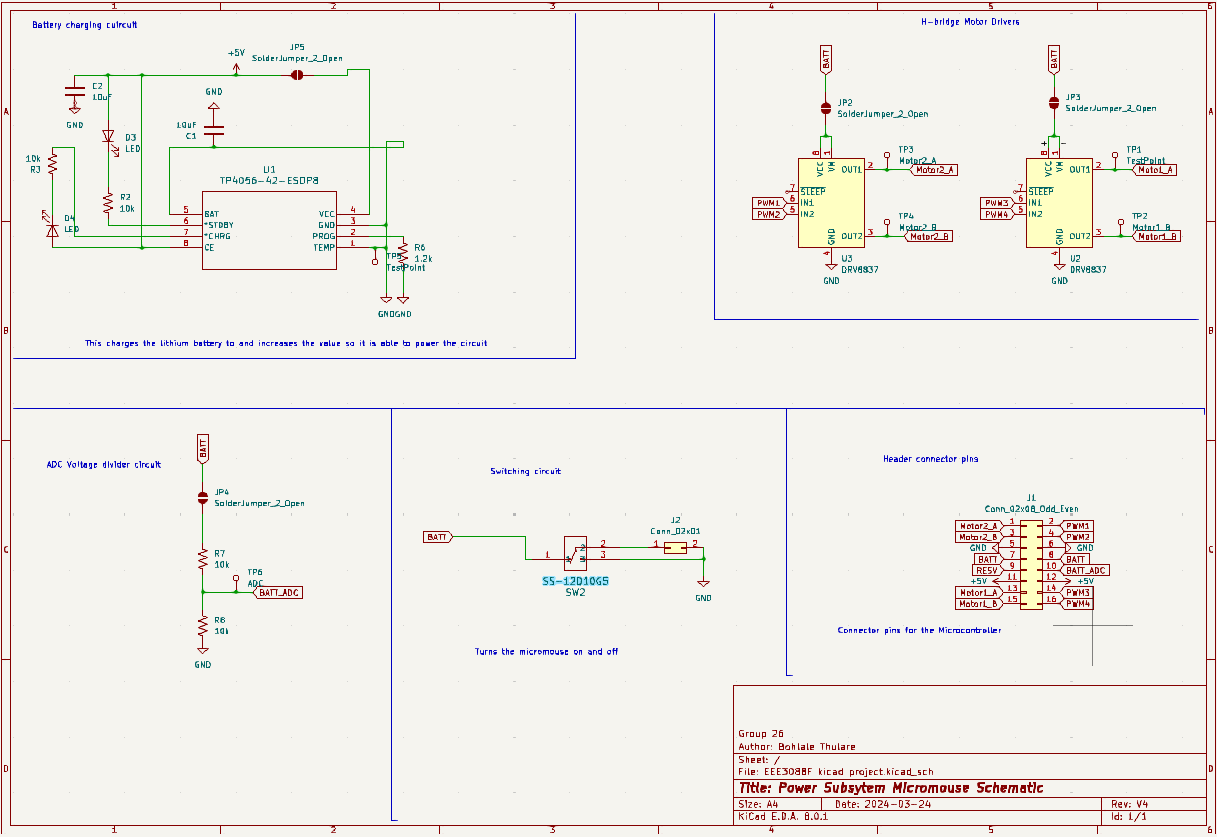
\includegraphics[width=0.5\linewidth]{EEE3088F_latex_template/Figures/schamatic.png}
    \caption{Schematic}
    \label{fig:schematic}
\end{figure}

\begin{figure}[h]
     \centering
    % First subfigure
    \begin{subfigure}[b]{0.3\linewidth}
        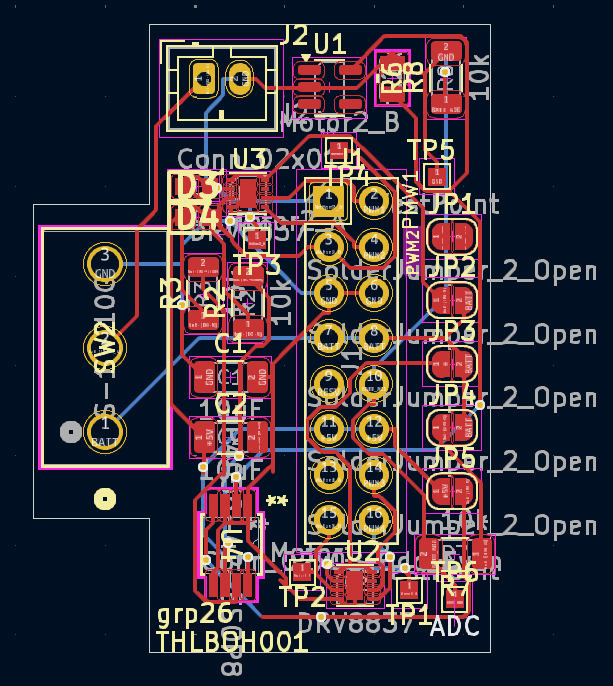
\includegraphics[width=\linewidth]{EEE3088F_latex_template/Figures/front.png}
        \caption{Front PCB}
        \label{fig:PCB_front}
    \end{subfigure}
    \hfill % Space between the subfigures
    % Second subfigure
    \begin{subfigure}[b]{0.3\linewidth}
        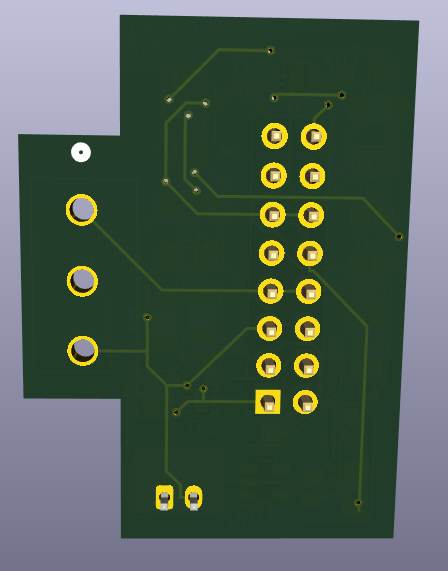
\includegraphics[width=\linewidth]{EEE3088F_latex_template/Figures/back.png}
        \caption{Back PCB}
        \label{fig:PCB_back}
    \end{subfigure}
    \hfill % Space between the subfigures
    % Third subfigure
    \begin{subfigure}[b]{0.3\linewidth}
        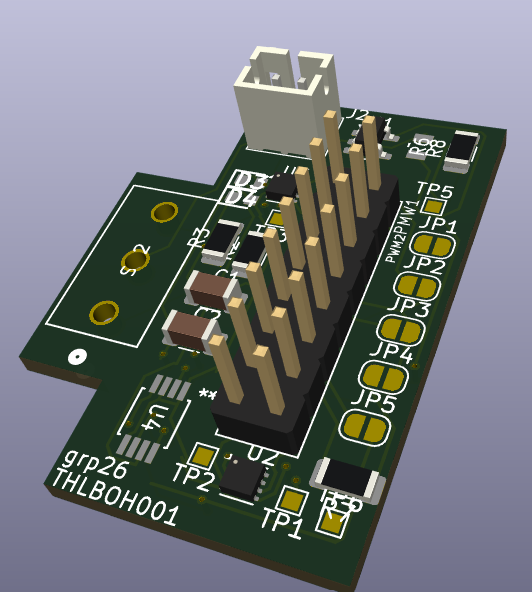
\includegraphics[width=\linewidth]{EEE3088F_latex_template/Figures/3d.png}
        \caption{3D PCB}
        \label{fig:PCB_3D}
    \end{subfigure}
    \caption{PCB}
    \label{fig:PCB}
\end{figure}
% =====================================================
\section{Failure Management}

\begin{table}[h]
    \centering
    \caption{Table of the failure management solutions used} \label{tab:failuremanagement}
    \begin{tabular}{|c|m{12cm}|}
        \hline
        \textbf{Name} & \textbf{Description} \\
        \hline
         Jumpers & Open jumpers are used ar the points in the circuitry that the designer is usure that the connection will work or will not damage the components. In this case the are used at input points of the different circuits \\
         \hline
         Test points  &  Test points are used to observe the state of the circuit at that point. This can be helpful with failure manegment by monitoring while testing to see what works and what would cause damage.  \\
         \hline
         Capacitor &  Allow cuurent to flow through a circuit gradually. This protects components from damage and helps with power distrubution.\\
         \hline
    \end{tabular}
\end{table}

% =====================================================
\section{System Integration and Interfacing}
To integrate the subsystem with the rest of the system ....
\\
\begin{table}[h]
  \begin{center}
    \caption{Interfacing specifications}
    \label{tab:Interfacing}
    \begin{tabular}{ >{\centering\arraybackslash}m{3cm}  m{5cm} m{7cm}}
      \hline
      \textbf{Interface} & \textbf{Description} & \textbf{Pins/Output} \\   
      \hline
      I001 & Power subsytem to STM board for continuous signal & \tabitem Connector pin14 to STM PC6-9 
      \newline\indent\tabitem Power subsystem to motor for diving \\
      \hline
      I002 & Power subsystem to motor for diving &\tabitem 1 and pin 3 to motor 2\\
      \hline 
      I003 & ower subsystem to motor for diving  & \tabitem Pin 15 and pin 13 to motor 1 \\
      \hline
    \end{tabular}
  \end{center}
\end{table}

\begin{figure}[h]
    \centering
    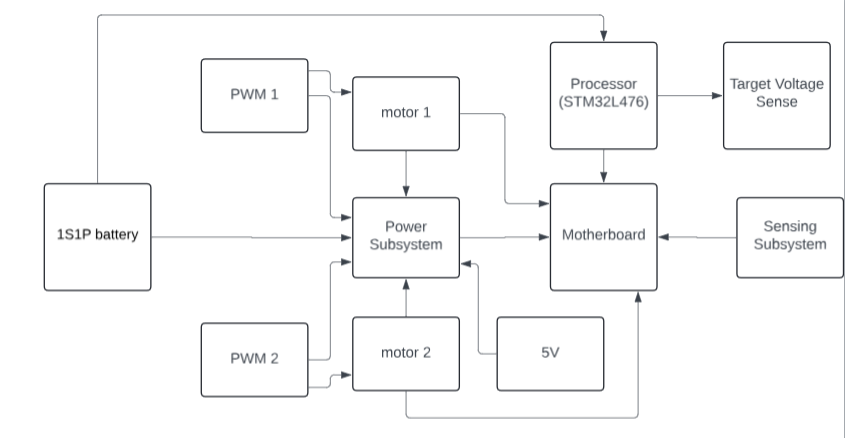
\includegraphics[width=0.5\linewidth]{EEE3088F_latex_template/Figures/context diagram.png}
    \caption{Context diagram}
    \label{fig:context diagram}
\end{figure}
% ----------------------------------------------------
\ifstandalone
\bibliography{../Bibliography/References.bib}
\fi
\end{document}
% ----------------------------------------------------